% -*- compile-command: "cd .. && make" -*-
\documentclass[document.tex]{subfiles}
\begin{document}

\chapter{Platform}
\label {ch:platform}

The results of the first case study were used to define a new platform for workflow-based web development on Rails. The intention is to provide programmers with a set of reusable components that allow them to perform common tasks required by workflow-based applications, without sacrificing usability.

AASM, Devise, and Pundit form the core of the new platform. These third-party libraries (or ``gems'' in Ruby parlance) cover the two key requirements of all workflow platforms: as workflows are sequences of steps carried out by one or more users in specific roles, then it is necessary for workflow-based applications to encode both the sequence of steps and the ability to recognize users and roles. AASM provides support for encoding sequences of steps using a domain-specific language for state machines, while Devise and Pundit provide the authentication and authorization required to identify users and slot them into specific roles. Stonepath itself is omitted from the platform as the initial prototype and following case study were unable to make use of its features, and instead only used AASM.

Several new libraries were also created to provide common workflow-related features as part of the platform. As illustrated by the package diagram in Figure \ref{fig:platform-package-diagram}, these new libraries build on the core third-party libraries in the platform.

Each new package is described in more detail in the following sections. The section for each package summarizes the motivation for including the package in the platform, presents a brief description of the package, and discusses how the package is tested.

\begin{figure}[!ht]
\centering 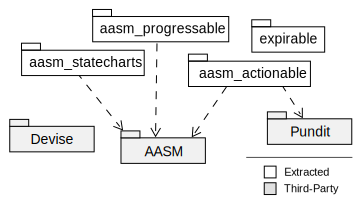
\includegraphics[width=4.5in]{./img/platform/platform-package-diagram}
\caption{Package diagram of the new workflow platform.}
\label{fig:platform-package-diagram}
\end{figure}

\FloatBarrier


\sectionnote {BM}
\section {aasm\_statecharts}

The AASM domain specific language provides a readable and writable way to define state machines in Ruby. Unfortunately, it is still less readable than graphical techniques such as state charts; developers cannot easily intuit the overall flow of events in a workflow from a textual description, but can if they are provided with a graphical representation.

While several tools exist to general state machine diagrams from AASM definitions, these tools do not express the full range of concepts supported by AASM. The existing tools can generate finite state machine diagrams from AASM descriptions, but the generated diagrams lack guards, actions, or other features of extended state machines or statecharts.

\verb!aasm_statecharts! \cite{aasm_statecharts} is a new utility designed to address these shortcomings. It can convert AASM workflows to any image format support by Graphviz. It can not only represent states and transitions, but also entry and exit actions, transition actions, and transition guards.

\verb!aasm_statecharts! is based on the diagram generating tool described in section \ref{sec:4ys-visualizing-workflows}, with some modifications to the structure of the code to improve testability. While the original diagram generator was implemented as a single Ruby script, \verb!aasm_statecharts! is split into two parts: a library module (\verb!lib/aasm_statechart.rb!) which implements the logic that maps from AASM to the Ruby-Graphviz object model, and a launcher script (\verb!bin/aasm_startecharts!) that handles parsing command line arguments and invoking the library module appropriately. This improves observability, as the test scripts can access the semantic information in the Ruby-GraphViz object model, instead of just the generated diagram.

Sufficient unit tests have been written to achieve 100\% coverage of the library module. The unit tests were written following a black-box methodology, following the testable characteristics of the parameters of the library methods.
% More detail about the tests can be found in section
% \ref{sec:platform-test-cases-aasm_statecharts}.
Note that the launcher script is still tested manually, as it is trivial to achieve full coverage of the command-line options in a few tests, and because the generated diagrams require human judgment to determine if they are correct.

\verb!aasm_statecharts! is available online at \url{https://github.com/WorkflowsOnRails/aasm_statecharts}, or it may be installed from the \verb!aasm_statecharts! gem.
A short manual is available on the project's GitHub page, and is also attached to this report in section \ref{sec:aasm-statecharts-manual}.


\sectionnote {BM}
\section {aasm\_progressable}
\label {sec:aasm-progressable}

Many workflow-based web applications present some indication of a user's progress through a workflow; for example, consider the registration workflow for GitHub presented in Figure \ref{fig:github-registration}. Such progress indicators are important for designing usable workflow-based user interfaces: they give users a sense of what to expect from future steps, as well as how much of the workflow they have completed.

\begin{figure}[!htbp]
  \centering
  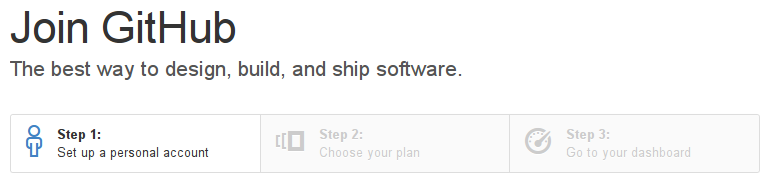
\includegraphics[width=6in]{./img/platform/github-registration}
  \cprotect
  \caption{Screenshot showing progress indicator used in GitHub's registration workflow. Note that step 1 is highlighted, indicating that it is the current step.}
  \label{fig:github-registration}
\end{figure}

Unfortunately, there is no existing off-the-shelf solution for rendering this type of progress indicator for a workflow implemented in AASM. Thus, the \verb!aasm_progressable! \cite{aasm_progressable} library was created to fill this gap. The library renders a progress indicator based on the current state of a model instance, plus an declaration in the model that specifies the order that the states are traversed in the workflow. The library follows Rails' conventions by separating the logic for computing completed states from the view that renders the progress bar, so that developers can customize the bar's appearance.

Although it might seem like the sequence of states could be inferred automatically, this is not the case; certain state machines have several possible natural orderings. Figure \ref{fig:equivalent-fsms}, presents one such state machine: while subfigure (a) appears to have state B precede state C, rearranging the diagram to yield (b) demonstrates that C could just as easily be inferred to come before B.

\begin{figure}[!htbp]
  \centering
  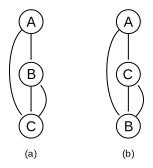
\includegraphics[width=2.3in]{./img/platform/equivalent-fsms}
  \cprotect
  \caption{Two representations of the same simplified finite state machine. (The transition labels have been removed for clarity.) The state machine depicted in (b) is equivalent to the one in (a), except nodes B and C have had their positions swapped.}
  \label{fig:equivalent-fsms}
\end{figure}

After extracting the library, a series of black-box tests were created in order to achieve more than 90\% statement coverage of the codebase. The exception to the test coverage is the \verb!AasmProgressable::Helper! module, which handles instantiating a few underlying classes, and passing them to a template to be rendered to HTML. The Rails testing libraries lack the ability to check the arguments passed to a call to \verb!render!, and while it would be possible to inject the helper module into a custom object and mock the \verb!render! method, this would be brittle and likely to fail if the code changed. Instead, the four lines in the method were left untested in the gem for now, as the results of rendering a progress indicator widget from the gem are already checked in the integration tests for the first case study.

\verb!aasm_progressable! can be found on GitHub at \url{https://github.com/WorkflowsOnRails/aasm_actionable}, and the stable version is available via the \verb!aasm_progressable! gem. A manual is available on the project's GitHub page, and is also reproduced in section \ref{sec:aasm-progressable-manual} of this report.

\FloatBarrier

\sectionnote {BM}
\section {aasm\_actionable}

Many steps in a workflow that require user interaction have the same form: the user selects which action they wish to perform, fills a form with some associated information, and submits the form to carry out the action. Using AASM, developers must still write the code necessary to present users with actions appropriate for the user's role and the current state of the workflow. This development effort is redundant, as the knowledge of which actions can be performed in the current state are already encoded in AASM, while Pundit captures information about who can perform which actions. In addition, duplicating this information makes applications less maintainable, as it now must be updated in two places if application requirements change.

\verb!aasm_actionable! \cite{aasm_actionable} is a library that allows developers to render actions automatically based on the information already captured by AASM and Pundit. The library is based on the technique described in section \ref{sec:4ys-available-actions}, which was extracted from the first case study. In addition to using \verb!StateActionRenderable! to automatically determine and render applicable actions, the library also includes a default container template (illustrated in Figure \ref{fig:aasm-actionable-example}) that renders each action in a separate tab. This template to helps developers get started more quickly with \verb!aasm_actionable! without having to create a container template that is specific to their application.

\begin{figure}[!htbp]
  \centering
  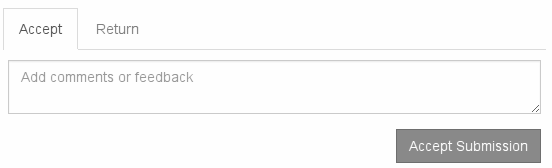
\includegraphics[width=5in]{./img/platform/aasm-actionable-example}
  \cprotect
  \caption{Screenshot showing the default template for \verb!aasm_actionable! in use in the fourth year project system. The template renders each action in a separate tab.}
  \label{fig:aasm-actionable-example}
\end{figure}

As with the other platform components, unit tests were written for \verb!aasm_actionable! until 100\% statement coverage was achieved for the controller mixins. Unfortunately, the default container template is only testable in Rails applications that include the library. Thus some basic rendering checks were incorporated into the integration tests in the fourth year project system in order to avoid setting up a new application solely to test the default view.

\verb!aasm_actionable! is available online at \url{https://github.com/WorkflowsOnRails/aasm_actionable}, or it may be installed from the \verb!aasm_actionable! gem.
A short manual is available on the project's GitHub page, and is also attached to this report in section \ref{sec:aasm-actionable-manual}.

\FloatBarrier


\sectionnote {BM}
\section {expirable}

Business processes often involve deadlines, such as ensuring that tax forms are prepared before the filing deadline, or support requests are answered within contractually-imposed time limits. Workflow frameworks must therefore support them as well -- however, AASM and Rails do not have such support out-of-the box, nor are there any third-party libraries that make it easy to implement deadlines for AASM.

\verb!expirable! \cite{expirable} is a Rails library that fills that gap. It uses the techniques described in section \ref{sec:4ys-handling-deadlines} to generate time-based events with Clockwork and then asynchronously run associated actions with \verb!Delayed::Job!. As the deadline-handling functionality was designed to be used by several models in the fourth year system, it was trivial to extract the reusable parts to a separate library without performing any refactoring.

Testing of the new gem was somewhat more complicated. Though the library's unit test suite achieved 100\% statement coverage of the code in the expirable library itself, the task of integration testing the library was complicated by the fact that \verb!Delayed::Job! runs in its own thread. This makes it difficult to detect when a deadline event has run from within the test runner without constructing an inter-process communication mechanism or polling the database. In the end the integration tests were omitted; based on the simplicity of the integration (which only involves invoking a ``delay'' method from \verb!Delayed::Job!) and the widespread use and excellent upstream test coverage, further test would add little value relative to the effort involved.

The completed library is available online at \url{https://github.com/WorkflowsOnRails/expirable}, or it may be installed from the \verb!expirable! gem.
A short manual is available on the project's GitHub page, and is also attached to this report in section \ref{sec:expirable-manual}.


%\sectionnote {BM}
%\section {Integration Testing the Platform}


\end{document}
